\chapter{Corpus Preparation}
\label{chap:corpus}
Since this research is based on a supervised learning algorithm, a high-quality corpus is essential to our success. In this chapter, we will review the existing corpora, various formats and specifications of a corpus, and how we construct the corpus used in this reasarch.

A expressive performance corpus is a set of performance samples. Each sample consists of a score and a recording. The score is simply the music score being played, which contains notational information; and the recording is a digital or audio recording of a human musician playing the said score. With the two elements, a learning algorithm can learn how the music notation is translated into real performance. These two elements can come in many format, in the next sections we will discuss the pros and cons of some possible candidate.
\section{Existing Corpora} 
There exist very few public accessable corpus on the Internet. CrestMusePEDB\cite{crestmuse} (PEDB stands for "(Music) Performance Expression Database", created by Japan Science and Technology Agency's CREST program, is one of the example. They claimed to have the following data in their database: PEDB-SCR - score text information, PEDB-DEV - performance deviation data and PEDB-IDX - audio performance credit. The database is free to use via email request. But until the time this thesis is written, the author can not get any response from the database andministrators, so the quality and format of the data is unknown.

Another example is the Magaloff Project\cite{magaloff} conducted by Flossmann et al., a joint effort from a few universities in Austria.  Russian pianist Nikita Magaloff recorded all works for solo piano by Frederic Chopin on a Bösendorfer SE, a computer-controlled grand piano. This corpus became the material for many subsequent researches \cite{magaloff extendedi}. Flossmann et al. also trained a expressive performance system call YQX\cite{yqx}, which won the 2008 RenCon contest, on this corpus. However, the corpus is not placed in the public domain. 

Without any public corpus available, we must record our own corpus, which will be discussed in detail in the next section.


\section{Score Representation}

There are many way to represent a music score in machine-readable format, such as MusicXML\cite{Good2001}, LilyPond\cite{LilyPond}, Finale, Sibelius, ABC, MuseData, and Humdrum. For more information, please check out \cite{Selfridge-Field1997}. For research purpose, proprietary format like Finale and Sibelius is abandoned because of their limited support from open source tools. MusicXML is based on XML (eXtensible Markup Language), it can express most music notations and metadata. LilyPond is a \LaTeX-like language for music typesetting. ABC, MuseData and Humdrum are based on ASCII codes and each defines their unique representation for music score. 
%TODO: guitar pro?
Other formats such as image files (scanned or typesetted by computer) or PDF files are an alternative, but they are not an option for direct computer analysis. MIDI can also be shown as music score in some music notation software, but MIDI is design as control signals for digital music equipments, so it lacks some music notations. Furthermore, the model of low-level music instrument control signals doesn't fit well with music notation, so it is not considered a good way to representation for music score.

In this research, we use MusicXML as the main vehicle for music score, because of the following reasons: first, it covers most music notations and metadata need for this research. Second, it is supported in most music notation software, including the one used in this research -- MuseScore. Finally, the music21 toolbox can convert many other formats into MusicXML without problem.
 
 %TODO:score example pic

\begin{figure*}[tp]
   \begin{center}
      %TODO:Figure:Example JSON code
      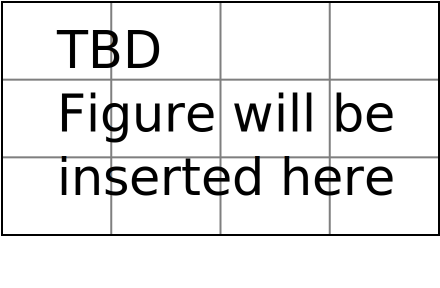
\includegraphics[width=\textwidth]{fig/TBDFigure}

   \end{center}
   \caption{Example MusicXML score}
   \label{fig:expxml}
\end{figure*}

\begin{figure*}[tp]
   \begin{center}
      %TODO:Figure:Example JSON code
      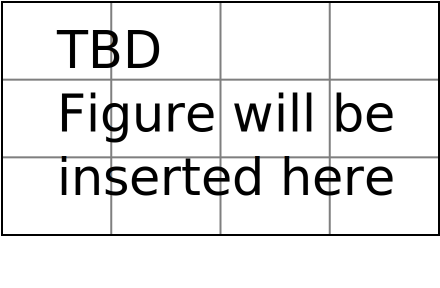
\includegraphics[width=\textwidth]{fig/TBDFigure}

   \end{center}
   \caption{Example MusicXML Score (Rendered)}
   \label{fig:expxmlrend}
\end{figure*}

\section{Recording Format}
A recording of expressive performance can be in MIDI or audio such as PCM WAV. Although audio recording has higher fidelity than MIDI, it takes extra effort to be analyzed by computer. Since onset detection and pitch detection algorithms still can't achieve perfect accuracy, manually labeling each notes required, which will soon become impossible to do when the texture of music become polyphonic. On the other hand, a multichannel MIDI recording can provide exact timing, key pressure, and pitch for each note, but it lacks timber and envelope information, which makes it hard to analyze how the musician use instrument-specific skills. Considering the above arguments, MIDI is used in this research.

A human musician can't play every note exactly on the beat, even if playing along with a metronome. There are two ways to record this behavior: first, record the exact note-on and note-off time, while keeping the tempo fixed; second, keep the notes on the beat, so the MIDI looks the same as the score. Then insert tempo-change event between each notes, so notes of the same length can be rendered differently because they have different tempo marker. The second method may look smart, because the score and performance can be stored in one MIDI file instead of two, but it would involve complex calculation when linearly scaling the tempo. Since tempos from different samples need to be normalized during feature extraction, the first method is superior  than the second.

 %TODO:recording example pic
\framebox{TODO: discuss how I do the phraseing}
\begin{figure*}[tp]
   \begin{center}
      %TODO:Figure:Example JSON code
      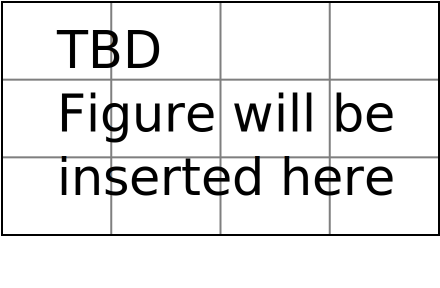
\includegraphics[width=\textwidth]{fig/TBDFigure}

   \end{center}
   \caption{Example Recording Compared to Score (Pianoroll)}
   \label{fig:exprecording}
\end{figure*}


\section{Specfication/Implementation}

Because of the limited ability of current implementation of our system, and the limited time and resource we have, we have to impose some constrain on the recordings:
\begin{enumerate}
   \item All the samples are monophonic. They only contain single line of melody, without chords.
   \item A song is divided into phrases by manually labeling.
   \item No human error exist in the recording; the score and recording are matched note-by-note.
   \item The tempo label in MIDI recordings are the tempo by which the musician played. 
\end{enumerate}

For our corpus, we choose Clementi's Sonatina Op. 36.  This is because  Clementi's Sonatina is a basic repertoire almost every piano student in Asia will learn, so it' s easy to find performers with different skill level to record the corpus. Clementi wrote these sonatinas in classical style, so the skill required to play them can be easily extended to other classical era works like Mozart or Haydn. This fact makes the learned model a very general one, which is good for evaluation.

The digital score used is downloaded from KernScore website \cite{KernScores}. The original format is in Hundrum file format (.krn), then transformed into MusicXML by music21 toolkit. Because this research focus on monophonic melody only, so the chords in the scores are manually reduced to the highest note in the chord, which is usually the most salient melody line. All the other possible errors in the downloaded score is manually corrected to make them ready for printing and computer analysis. We use MuseScore notation editor to view and edit MusicXML; some metadata errors are corrected by editing the MusicXML with text editors .

\framebox{TODO: early version: touch pad recordings}
To record the MIDI performances, we used a Yamaha MIDI keyboard with pressure sensitive keys. The Yamaha keyboard was connected to a MIDI-to-USB  converter so it acted as a USB MIDI device on our Linux computer. On the Linux computer the Rosegarden Digital Audio Workstation (DAW) is used to record the MIDI. The Rosegarden DAW also generated the metronome sound to help the performer maintain a steady speed. One may argue that the tempo variation is also a part of the expression, but if the performer plays freely, the tempo is hard to determine afterwards, which will make learning scaling the performance in time domain very hard. So the performers are asked to follow the speed of the metronome, but they can apply any level of rubato as they like. The performers were allowed to record multiple times and edit the recording until there were no mistakes. The human error model is not part of this research now, so no mistakes are allowed in the performances to keep the problem simple.

  After the MIDIs are recorded, some utility scripts we wrote are employed to  make sure each recording is matched note-to-note with the corresponding score; if not, we will manually correct those mistakes. For example, if the pitch was played wrongly, we will correct the pitch but keep the onset, duration  and intensity as is. The matched score and MIDI pair are then splat into phrases according to a phrasing file.  Each line in the phrasing file is the starting point of each phrase. The starting point is defined as the onset timing (in quarter notes) of the first note in a phrase in the score.  The phrasing is assigned by the researcher now for accuracy, but any phrasing algorithm can be applied.

  \framebox{Discuss the pre-split check, split script, post-split check, corpus preparation scirpt, etc.}

  \framebox{TODO: discuss how to specify the phrase if the phrase start at 1/3 position}

 %TODO: phrase file example
\begin{figure*}[tp]
   \begin{center}
      %TODO:Figure:Example JSON code
      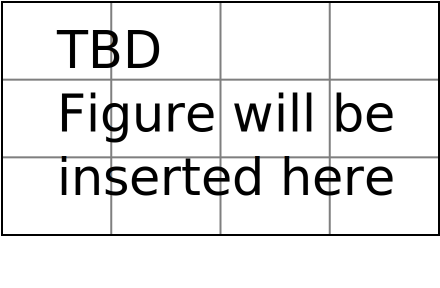
\includegraphics[width=\textwidth]{fig/TBDFigure}

   \end{center}
   \caption{Example Phrase File}
   \label{fig:phrase}
\end{figure*}


%TODO: corpus size, songs count, phrases count. reportie list
The coupus used in this research is recorded by five graduate students, with a wide range of piano skill. A total of (TBD) movements of Clementi's Sonatina is recorded, which contains (TBD) phrases, equals to (TBD) notes. 

Because of the scope of the research, we didn't use all the information available, here are a few pieces of potentially useful information:
\begin{enumerate}
   \item Polyphonic recording can provide information for polyphonic performance
   \item The gaps between phrases can be learned to create models for inter-phrase delay.
   \item Recordings with human error can make the system play more like human.
\end{enumerate}

\framebox{TODO: distribution of corpus}
